% +------------------------------------------------------------------------+
% | Reference manual chapter: overlay_ref.tex (Map Overlay)
% +------------------------------------------------------------------------+
% | 
% | Package: ovl (Map Overlay)
% | 
% +------------------------------------------------------------------------+

%+----------------------------------------------------------------------------80
%| update log
%|
%| 01 April 2002 - Eti Ezra
%|    Separated from intro.tex (See previous changes in change log there).
%|     
%+----------------------------------------------------------------------------80


% +========================================================================+
%   Introduction
% +========================================================================+
%\clearpage
%\section{Reference Pages for 2D Planar Maps}

\chapter{2D Map Overlays}
\label{chap:intro_ref}
\ccRefLabel{Ovl_intro}
\section{Introduction}

Given two planar subdivisions $R$ and $B$, 
the overlay of $R$ and $B$, 
denoted by $O(R,B)$, is the subdivision of the plane 
induced by the edges of $R$ and $B$.
We refer to the components of $R$ as red, 
and to the components of $B$ as blue.
$R$ and $B$ are also called the {\em creators} of $O(R,B)$.
The overlay $O(R,B)$ consists of all non-empty sets $r \cap b$, 
such that $r \in R$ and $b \in B$. 
Every such non-empty set in $O(R,B)$ maintains 
pointers to the components $r \in R$ and $b \in B$ that created it.
More specifically, if a component $o \in O(R,B)$ points 
to the respective components $r \in R$ and $b \in B$, 
we say that $r$ and $b$ lie {\em above} $o$, 
alternatively, we say that $o$ lies {\em below} $r$ and $b$.
Figure~\ref{OVL_sec:overlay_example} displays an overlay 
of two given rectangles.

We can divide the problem of computing $O(R,B)$ into two subproblems:
\begin{itemize}
\item reporting all intersections between $R$ and $B$.
This subproblem is related to the red-blue curve intersection 
problem: Given a set of non-intersecting red curves and a 
set of non-intersecting blue curves in the plane, 
with a total of $N$ curves, report all $k$ intersections of 
red curves and blue curves.
In our implementation we construct the arrangement of the 
red and the blue curves by two possible algorithms:
the {\it incremental} algorithm and the {\it sweep-line} 
algorithm (See section~\ref{sec:algorithms}. 
In the implementation of the incremental algorithm 
we use the \ccStyle{Planar_Map_with_Intersections} class 
in order to represent the arrangement in construction,
and in our implementation to the sweep-line algorithm 
we simply use the \ccc{Sweep_Line_2} package.
In the latter case we use a \ccStyle{Planar_map_2} class
in order to represent the arrangement in construction.

\item updating each component $o \in O(R,B)$ to point to the 
respective components of $R$ and $B$ that created it.
This subproblem is easier than the former one,
and can be solved by a single pass on the arrangement 
constructed in the former stage.
In our implementation, we define a special \ccStyle{DCEL}
for the \ccc{Map_Overlay_2} package,
which is the data structure representing the constructed arrangement 
induced by the overlay (see Section~\ref{sec:dcel}).
In addition, we use the \ccStyle{Map Overlay Notifier} 
(see Section\ref{sec:notifier}), which is 
a newly defined class containing methods for updating the pointers 
in each component of the DCEL representing the 
constructed arrangement.
\end{itemize}

\begin{figure}[h]
    \begin{ccTexOnly}
        \centerline{
           \includegraphics{./Map_overlay_2/overlay_example.eps}
           }
    \end{ccTexOnly}
    \caption{Two rectangles (left) and their overlay (right). 
       We denote the subdivision induced by the first rectangle by $R$ and the second by $B$. 
       The face $f$ of the overlay is below $f_1$ and the unbounded face of $B$. 
       The halfedge $e$ of the overlay contains a halfedge pointer to $e_2$ and two face pointers 
       to $f_1$ and to $f_2$ (note that $e$ lies in the interior of $f_1$). 
       The vertex $v$ of the overlay points to $v_2$, contains a halfedge 
       pointer to $e_2$ and lies below $f_1$ and $f_2$.}
    \label{fig:overlay_example}
\end{figure}


\begin{ccTexOnly}

\section{Software Design}
The \ccc{Map_overlay_2<Subdivision,Notifier>} class 
is a data structure for maintaining 2D map overlays.
The data structure maintains the subdivision induced by overlaying 
the two creators, and the two pointers to these creators. 
The underlying combinatorial structure is determined by
(i) {\it Subdivision} which presents the subdivision type 
representing the overlay and its two creators. 
{\it Subdivision} can be either \ccStyle{Planar_Map_2} or, 
 \ccStyle{Planar_Map_With_Intersections_2}.
% or an a \ccc{Arrangement}.
Notice that the choice of a subdivision type determines the choice 
of a DCEL and a traits class (see Chapter~\ccRefPage{I1_ChapterPlanarMap}).
(ii) {\it Notifier} is the class used to update the overlay components. 
{\it Notifier} should be a model of the 
\ccc{PlanarMapWithIntersectionsChangeNotification_2} concept.

\section{Map Overlay Algorithms}
\label{sec:algorithms}
The input to our algorithms are two planar subdivisions, 
$R$ and $B$, having $N$ curves in total. 
The overlay of $R$ and $B$ has $O(N+k)$ vertices, 
where $k$ is the number of intersections between $R$ and $B$.
The combinatorial complexity of the overlay may be quadratic 
in the size of $R$ and $B$ in the worst case.

We devised and implemented two algorithms for constructing the 
arrangement induced by $R$ and $B$.
The first algorithm is the {\em incremental} algorithm, 
and its complexity is near-quasratic in $N$. 
The second algorithm is a {\em sweep-line} algorithm 
for general curves, and its complexity is $O(N\log{N} + k\log{N})$.

In most cases, the sweep-line algorithm has much better performance 
than the incremental algorithm. Hence, users are encouraged employing 
the sweep-line algorithm,

\section{Map Overlay DCEL}
\label{sec:dcel}
The \ccc{Map_overlay_default_dcel<Traits,Vertex_base,Halfedge_base,Face_base>}
class is the data structure representing the DCEL of the overlay. 
We denote the above DCEL by $OD$.
The basic components of the DCEL representing the overlay are built 
on top of the basic components of the \ccStyle{Planar_Map_2} or 
the \ccStyle{Planar_Map_With_Intersections_2} 
(depending on the subdivision choosen in 
order to represent the overlay and its two creators).

The additional information we maintain in the components of the DCEL 
is the pointers to the components of the creators $R$ and $B$.
Namely, every component $o \in O(R,B)$ points to the 
respective components $r \in R$ and $b \in B$ that created it. 


\section{Map Overlay Notifier}
\label{sec:notifier}
Updating the DCEL additional attributes is performed by the {\em Notifier} class.
We extend and override the notification functions of the basic {\em Notifier}, 
defined in the \ccc{Planar_Map_2<Dcel,Traits>} package 
(see Chapter~\ccRefPage{I1_ChapterPlanarMap}), 
in order to update the corresponding features constructed by the overlay. 

\section{Boolean Operations:}
A straightforward usage of the \ccc{Map_overlay_2<Subsection,Notifier>} 
utilities, is performing boolean operations on planar subdivisions in general, 
and specifically on polygons.

An object of the \ccc{Boolean_operations_2<Map_Overlay>} class is initialized with 
two input subdivisions. In the initialization step, it constructs the overlay 
of the two input subdivisions. By constructing the overlay, all boolean operations, 
on the two input subdivisions, can be easily provided.
The  \ccc{Boolean_operations_2<Map_Overlay>} class provides methods for 
performing an intersection, union, symmetric difference and difference on the two 
input subdivisions. 
The output of such operations are all resulting vertices, halfedges and faces.


\subsection*{Polygons Bops:}
One of the most natural usage of 
the \ccc{Map_overlay_2<Subsection,Notifier>} utilities, 
is performing boolean operations on polygons.

The above utility is a straightforward usage of the 
\ccc{Boolean_operations_2<Map_Overlay>} 
class. Hence, every operation obtained from the functions 
for boolean operations on polygons can be achieved by 
directly using the \ccc{Boolean_operations_2<Map_Overlay>} 
class. 

The goal of providing these functions, is to 
provide a simple interface for users who are 
interested only in boolean operations on 
polygons, rather than boolean operations 
on planar subdivisions of general curves.

In our interface, we provide four function objects 
for all kinds of boolean operations on polygons,
namely, for intersection, union, difference, and 
symmetric difference.


\subsection*{Example: Overlaying Two Subdivisions of Line Segments:}
The following example demonstrates a simple usage of the 
\ccc{Map_overlay_2<Subdivision,Notifier>} package.
In this example we construct two planar maps of line segments. 
Then we construct their overlay using the sweep-line algorithm, which is 
the default algorithm for the overlay construction. 
After the overlay is constructed, we write its corresponding planar map to the 
standard output stream. 

\ccIncludeExampleCode{Map_overlay_2/example1.C}
The input of the program is a text file containing two lists of segments, 
each of which represents an input subdivision.
\ccIncludeExampleCode{Map_overlay_2/example1.cin}

The output of the program looks like this:
\ccIncludeExampleCode{Map_overlay_2/example1.cout}


\subsection*{Concepts}
\ccRefConceptPage{MapOverlayDcel_2}\\
\ccRefConceptPage{MapOverlayDcelVertex_2}\\
\ccRefConceptPage{MapOverlayDcelHalfedge_2}\\
\ccRefConceptPage{MapOverlayDcelFace_2}\\
\ccRefConceptPage{MapOverlayAlgorithm_2}\\
\ccRefConceptPage{MapOverlayNotifier_2}\\
\ccRefConceptPage{PolygonBopsTraits_2}\\

\subsection*{Classes}
\ccRefIdfierPage{CGAL::Map_overlay_2<Subdivision,Notifier>}\\
\ccRefIdfierPage{CGAL::Map_overlay_default_dcel<Traits,V,H,F>}\\
\ccRefIdfierPage{CGAL::Map_overlay_incremental<Subdivision,Notifier>}\\
\ccRefIdfierPage{CGAL::Map_overlay_sweep<Subdivision,Notifier>}\\
\ccRefIdfierPage{CGAL::Map_overlay_default_notifier<Subdivision>}\\
\ccRefIdfierPage{CGAL::Boolean_operations_2<Map_overlay>}\\
\ccRefIdfierPage{CGAL::Polygons_do_intersect_2<Traits>}\\
\ccRefIdfierPage{CGAL::Polygons_intersection_2<Traits>}\\
\ccRefIdfierPage{CGAL::Polygons_union_2<Traits>}\\
\ccRefIdfierPage{CGAL::Polygons_difference_2<Traits>}\\
\ccRefIdfierPage{CGAL::Polygons_symmetric_difference_2<Traits>}\\
\end{ccTexOnly}    







